\documentclass[10pt]{beamer}
\usepackage[utf8]{inputenc}

\usetheme{metropolis}

\usepackage{acronym} % \ac[p], \acl[p], \acs[p], \acf[p]
\usepackage{appendixnumberbeamer}
\usepackage[scale=2]{ccicons}
\usepackage{subcaption} % subfigure
\usepackage[absolute, overlay]{textpos}
\usepackage{tikz}
\usetikzlibrary{positioning}
\usetikzlibrary{calc}
\usetikzlibrary{shapes.misc}
\usepackage{verbatim}

\usepackage{transparent}

\usepackage{graphicx}
\usepackage{color}
\AtBeginDocument{
\definecolor{pdfurlcolor}{rgb}{0,0,0}
\definecolor{pdfcitecolor}{rgb}{0,0,0}
\definecolor{pdflinkcolor}{rgb}{0,0,0}
\definecolor{light}{gray}{.85}
\definecolor{vlight}{gray}{.95}
\definecolor{darkgreen}{RGB}{77,172,38}
\definecolor{darkblue}{RGB}{5,113,176}
\definecolor{mydarkblue}{RGB}{116,173,209}
\definecolor{mydarkblueid}{RGB}{83,154,198}
\definecolor{mylightblue}{RGB}{171,217,233}
\definecolor{mydarkorange}{RGB}{244,109,67}
\definecolor{mylightorange}{RGB}{252,153,54}
\definecolor{mydarkred}{RGB}{215,48,39}
\definecolor{mydarkpurple}{RGB}{140,107,177}
\definecolor{mydarkpurpleid}{RGB}{136,86,167}
}

% Acronyms
% --------
\acrodef{CRDT}[CRDT]{Conflict-free Replicated Data Type}
\acrodefplural{CRDT}[CRDTs]{Conflict-free Replicated Data Types}

\author{
  \textbf{Matthieu Nicolas} (\url{matthieu.nicolas@loria.fr}), Gérald Oster, Olivier Perrin
  \\
  COAST team
}
\title{Efficient renaming in Conflict-free Replicated Data Types (CRDTs)}
\subtitle{Case Study of a Sequence CRDT : LogootSplit}
\institute{
  \vspace{3em}
  \includegraphics[width=2.8cm]{img/loria-logo.png}\hspace{3em}
  \includegraphics[width=1.2cm]{img/ul-logo.pdf}\hspace{3em}
  \includegraphics[width=3cm]{img/inria-logo.pdf}\hspace{3em}
  \includegraphics[width=1.2cm]{img/cnrs-logo.png}
}

\usepackage[backend=biber,defernumbers=true,style=trad-plain,sorting=ydnt,maxbibnames=1,maxcitenames=1]{biblatex}
\addbibresource{biblio.bib}
\AtBeginBibliography{\footnotesize}
\setbeamertemplate{bibliography item}[text] % use ref number in bibliography

\renewcommand{\thefootnote}{[\arabic{footnote}]}
\newcommand{\trm}[1]{\mathit{#1}}
\newcommand{\id}[3]{$\trm{#1}^{\trm{#2}}_{\trm{#3}}$}
\newcommand{\epoch}[1]{$\varepsilon_{#1}$}


\newcommand{\widthletter}{2em}
\newcommand{\widthblock}{3em}
\newcommand{\widthoriginepoch}{1.65em}
\newcommand{\widthepoch}{1.8em}

% Tikz styles
\tikzset{
    common/.style={anchor=west, draw, rectangle, minimum height=6mm},
    letter/.style={common, minimum width=\widthletter},
    block/.style={common, minimum width=\widthblock},
    epoch/.style={letter, rounded rectangle, rounded rectangle east arc=0pt, minimum width=\widthepoch},
    point/.style={insert path={ node[scale=5*sqrt(\pgflinewidth)]{.} }},
    op/.style={draw, circle, minimum size=2.7em},
    cross/.style={
        path picture={
            \draw[mydarkred, very thick]
                (path picture bounding box.south east)--(path picture bounding box.north west)
                (path picture bounding box.south west)--(path picture bounding box.north east);
        }
    },
    invisible/.style={opacity=0},
    visible on/.style={alt=#1{}{invisible}},
    alt/.code args={<#1>#2#3}{%
      \alt<#1>{\pgfkeysalso{#2}}{\pgfkeysalso{#3}} % \pgfkeysalso doesn't change the path
    },
}

\usepackage{silence}
\WarningFilter{biblatex}{Patching footnotes failed}

\begin{document}

\begin{frame}[t,plain]
  \maketitle
\end{frame}

\begin{frame}{\acfp{CRDT} \footfullcite{shapiro_2011_crdt}}
  \begin{columns}
    \begin{column}{0.65\textwidth}
      \begin{tikzpicture}

        \node (origin) {};
        \path (origin)
          to ++(90:2) node[label=below:{\textbf{A}},
            label=above:{
              \includegraphics<1>[scale=0.5]{img/doc.pdf}
              \includegraphics<2-4>[scale=0.5]{img/docA.pdf}
              \includegraphics<5->[scale=0.5]{img/docABC.pdf}}
          ] (A) {\includegraphics{img/blue-node.pdf}};

        \path (origin)
          to ++(225:2) node[label=below:{\textbf{B}},
            label=left:{
              \includegraphics<1-2>[scale=0.5]{img/doc.pdf}
              \includegraphics<3>[scale=0.5]{img/docA.pdf}
              \includegraphics<4>[scale=0.5]{img/docAB.pdf}
              \includegraphics<5>[scale=0.5]{img/docABC.pdf}
            }] (B) {\includegraphics{img/red-node.pdf}};

        \path (origin)
          to ++(-45:2) node[label=below:{\textbf{C}},
            label=right:{
              {\transparent{0.4}\includegraphics<1-3>[scale=0.5]{img/doc.pdf}}
              \includegraphics<4>[scale=0.5]{img/docC.pdf}
              \includegraphics<5->[scale=0.5]{img/docABC.pdf}
            }] (C) {
              {\transparent{0.4}\includegraphics<1-3>{img/green-node.pdf}}
              \includegraphics<4->{img/green-node.pdf}
              };

        \draw (A) -- (B) -- (C) -- (A);

        \node<2>[below left=-30pt and 5pt of A] {\includegraphics[scale=0.4]{img/blue-update.pdf}};
        \node<2, 4>[below right=-30pt and 5pt of A] {\includegraphics[scale=0.4]{img/blue-update.pdf}};

        \node<4>[below right=-4pt and 1pt of B] {\includegraphics[scale=0.5]{img/red-update.pdf}};
        \node<4>[above left=1pt and -15pt of B] {\includegraphics[scale=0.5]{img/red-update.pdf}};

        \node<4>[below left=-4pt and 1pt of C] {\includegraphics[scale=0.5]{img/green-update.pdf}};
        \node<4>[above right=1pt and -15pt of C] {\includegraphics[scale=0.5]{img/green-update.pdf}};
      \end{tikzpicture}
    \end{column}
    \begin{column}{0.35\textwidth}
      \begin{itemize}
        \item Replicated data structure
        \item<2-> Updates performed without coordination
        \item<5-> Strong Eventual Consistency
      \end{itemize}
    \end{column}
  \end{columns}
\end{frame}

\begin{frame}{LogootSplit \footfullcite{AndreCollaborateCom2013}}
  \begin{itemize}
    \item State of the art of \emph{Sequence \acp{CRDT}}
    \item Elements are ordered by their identifier, noted here with the following formalism: \id{position}{node\_id~node\_seq}{offset}
  \end{itemize}

  \pause

  \begin{columns}
    \begin{column}{0.33\textwidth}
      \begin{figure}
        \centering
        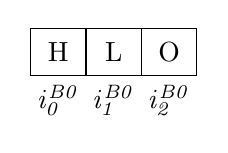
\begin{tikzpicture}
            \path
                node[letter, label=below:{\id{i}{B0}{0}}] {H}
                to ++(0:\widthletter) node[letter, label=below:{\id{i}{B0}{1}}] {L}
                to ++(0:\widthletter) node[letter, label=below:{\id{i}{B0}{2}}] {O};
        \end{tikzpicture}
        \caption{State of a sequence which contains the elements "hlo" and their corresponding identifiers}
      \end{figure}
    \end{column}
    \pause
    \begin{column}{0.33\textwidth}
      \vspace{-9mm}
      \begin{figure}
        \centering
        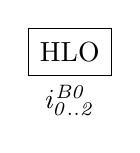
\begin{tikzpicture}
            \path
                node[block, label=below:{\id{i}{B0}{0..2}}] {HLO};
        \end{tikzpicture}
        \caption{State of a sequence which contains the block "hlo"}
      \end{figure}
    \end{column}
    \pause
    \begin{column}{0.33\textwidth}
      \begin{figure}
        \vspace{-7mm}
        \centering
        \begin{tikzpicture}
            \path
              node[letter, label=below:{\id{i}{B0}{0}}] {H}
              to ++(0:\widthletter) node[letter, fill=mydarkorange, label=above:{\color{mydarkorange}\id{i}{B0}{0}\id{f}{A0}{0}}] {E}
            to ++(0:\widthletter) node[block, label={below:\id{i}{B0}{1..2}}] {LO};
        \end{tikzpicture}
        \caption{State of a sequence which contains the elements "hlo" and their corresponding identifiers}
      \end{figure}
    \end{column}
  \end{columns}
\end{frame}

\begin{frame}{Research issue}

  \begin{itemize}
    \item \textbf{Evergrowing overhead:} impacts memory, bandwidth and CPU
  \end{itemize}

  \begin{columns}
    \begin{column}{0.45\textwidth}
      \begin{figure}
        \centering
        \includegraphics[width=\textwidth]{img/overhead-size.pdf}
        \caption{Memory footprint of the data structure}
      \end{figure}
    \end{column}
    \begin{column}{0.55\textwidth}
      \begin{itemize}
        \item \textbf{Operation count:} 100k
        \item \textbf{Size of content:} 100KB
        \item \textbf{Size of data structure:} 20MB
      \end{itemize}
    \end{column}
  \end{columns}

  \centering
  \alert{How to reduce the overhead introduced by the data structure?}
\end{frame}

% \begin{frame}[standout]
%   \alert{How to reduce the overhead introduced by the data structure ?}

%   \bigskip
%   \pause

%   Reassign shorter identifiers in a fully distributed manner
% \end{frame}

\begin{frame}[standout]
  \alert{Our approach}

  \bigskip

  Reassign shorter identifiers and aggregate them into blocks in a fully distributed manner
\end{frame}

\begin{frame}{RenamableLogootSplit}
  \begin{itemize}
    \item Propose \emph{RenamableLogootSplit}, \emph{LogootSplit} with a $rename$ operation
    \item Can be performed without coordination
  \end{itemize}
  \begin{figure}
    \includegraphics<1>{img/rename-op-initial-state.pdf}
    \includegraphics<2>{img/rename-op-first-id.pdf}
    \includegraphics<3>{img/rename-op-remaining-ids.pdf}
    \includegraphics<4>{img/rename-op-final-state.pdf}
    \caption{Example of renaming}
  \end{figure}
  \begin{itemize}
    \item<2-> Generates a new identifier for the first element, based on its previous identifier
    \item<3-> Then generates contiguous identifiers for all following elements
  \end{itemize}
\end{frame}

% \begin{frame}{Handling concurrent operations - part 1}
%   \begin{itemize}
%     \item Others may perform updates concurrently to a \emph{rename} operation
%   \end{itemize}
%   \begin{figure}
%     \centering
%     \includegraphics<1>[scale=0.75]{img/concurrent-op-initial-state.pdf}
%     \includegraphics<2>[scale=0.75]{img/concurrent-op-before-applying.pdf}
%     \includegraphics<3>[scale=0.75]{img/concurrent-op-inconsistency.pdf}
%     \caption{Example of concurrent insert}
%   \end{figure}
%   \begin{itemize}
%     \item<3> May lead to inconsistencies
%   \end{itemize}
% \end{frame}

\begin{frame}{Handling concurrent operations}
  \begin{figure}
    \centering
    \resizebox{\columnwidth}{!}{%
      \begin{tikzpicture}
          \path
              node {\textbf{A}}
              to ++(0:\widthletter) node[letter, label=below:{\id{i}{B0}{0}}] {H}
              to ++(0:\widthletter) node[letter, fill=mydarkorange, label=above:{\color{mydarkorange}\id{i}{B0}{0}\id{f}{\,A0}{0}}] {E}
              to ++(0:\widthletter) node[block, label=below:{\id{i}{B0}{1..2}}] (S0A-right) {LO}
              to ++(0:5 * \widthletter) node[block, fill=mydarkblue,
                      label={below:{\color{mydarkblueid}\id{i}{A1}{0..3}} }
                          ] (S1A) {HELO}
              to ++(0:8 * \widthletter) node[invisible, block, fill=mydarkblue,
                      label={[invisible]below:{\color{mydarkblueid}\id{i}{A1}{0..3}} }
                          ] (S2A-left) {HELO}
              to ++(0:\widthblock) node[invisible, letter, fill=mylightorange, cross,
                      label={[invisible] above:{\color{mylightorange}\id{i}{B0}{0}\id{m}{B1}{0}} }
                          ] {L};

          \path
              to ++(270:2) node {\textbf{B}}
              to ++(0:\widthletter) node[letter, label=below:{\id{i}{B0}{0}}] {H}
              to ++(0:\widthletter) node[letter, fill=mydarkorange, label=above:{\color{mydarkorange}\id{i}{B0}{0}\id{f}{\,A0}{0}}] {E}
              to ++(0:\widthletter) node[block, label=below:{\id{i}{B0}{1..2}}] (S0B-right) {LO}
              to ++(0:5 * \widthletter) node[invisible, letter, label={[invisible] below:{\id{i}{B0}{0}}}] (S1B-left) {H}
              to ++(0:\widthletter) node[invisible, letter, fill=mydarkorange, label={[invisible] above:{ \color{mydarkorange}\id{i}{B0}{0}\id{f}{\,A0}{0}}}] {E}
              to ++(0:\widthletter) node[invisible, letter, fill=mylightorange, label={[invisible] below:{ \color{mylightorange}\id{i}{B0}{0}\id{m}{B1}{0}}}] {L}
              to ++(0:\widthletter) node[invisible, block, label={[invisible] above:{\id{i}{B0}{1..2}}}] (S1B-right) {LO};


          \draw[->, thick] (S0A-right) -- node[above, align=center]{\emph{rename}} (S1A);
          \draw[invisible, dotted] (S1A) -- (S2A-left);
          \draw[invisible, ->, thick] (S0B-right) -- node[below, align=center]{\emph{insert "L"}\\\emph{between}\\\emph{"E" and "L"}} (S1B-left);
          \draw[invisible, dashed, ->, thick, shorten >= 3] (S1B-right.east) -- node[below right, align=center]{\emph{insert "L" at} {\color{mylightorange}\id{i}{B0}{0}\id{m}{B1}{0}}} (S2A-left.west);

      \end{tikzpicture}
    }
    \caption{Example of concurrent update}
  \end{figure}
  \vspace{-3mm}
  \begin{itemize}
    \item Can issue operations concurrently to \emph{rename}
    \item Produce inconsistencies if applied naively
  \end{itemize}
\end{frame}

\begin{frame}{Handling concurrent operations}
  \begin{figure}
    \centering
    \resizebox{\columnwidth}{!}{%
      \begin{tikzpicture}
          \path
              node {\textbf{A}}
              to ++(0:\widthletter) node[letter, label=below:{\id{i}{B0}{0}}] {H}
              to ++(0:\widthletter) node[letter, fill=mydarkorange, label=above:{\color{mydarkorange}\id{i}{B0}{0}\id{f}{\,A0}{0}}] {E}
              to ++(0:\widthletter) node[block, label=below:{\id{i}{B0}{1..2}}] (S0A-right) {LO}
              to ++(0:5 * \widthletter) node[block, fill=mydarkblue,
                      label={below:{\color{mydarkblueid}\id{i}{A1}{0..3}} }
                          ] (S1A) {HELO}
              to ++(0:8 * \widthletter) node[invisible, block, fill=mydarkblue,
                      label={[invisible]below:{\color{mydarkblueid}\id{i}{A1}{0..3}} }
                          ] (S2A-left) {HELO}
              to ++(0:\widthblock) node[invisible, letter, fill=mylightorange, cross,
                      label={[invisible] above:{\color{mylightorange}\id{i}{B0}{0}\id{m}{B1}{0}} }
                          ] {L};

          \path
              to ++(270:2) node {\textbf{B}}
              to ++(0:\widthletter) node[letter, label=below:{\id{i}{B0}{0}}] {H}
              to ++(0:\widthletter) node[letter, fill=mydarkorange, label=above:{\color{mydarkorange}\id{i}{B0}{0}\id{f}{\,A0}{0}}] {E}
              to ++(0:\widthletter) node[block, label=below:{\id{i}{B0}{1..2}}] (S0B-right) {LO}
              to ++(0:5 * \widthletter) node[letter, label={below:{\id{i}{B0}{0}}}] (S1B-left) {H}
              to ++(0:\widthletter) node[letter, fill=mydarkorange, label={above:{ \color{mydarkorange}\id{i}{B0}{0}\id{f}{\,A0}{0}}}] {E}
              to ++(0:\widthletter) node[letter, fill=mylightorange, label={ below:{ \color{mylightorange}\id{i}{B0}{0}\id{m}{B1}{0}}}] {L}
              to ++(0:\widthletter) node[block, label={ above:{\id{i}{B0}{1..2}}}] (S1B-right) {LO};


          \draw[->, thick] (S0A-right) -- node[above, align=center]{\emph{rename}} (S1A);
          \draw[invisible, dotted] (S1A) -- (S2A-left);
          \draw[->, thick] (S0B-right) -- node[below, align=center]{\emph{insert "L"}\\\emph{between}\\\emph{"E" and "L"}} (S1B-left);
          \draw[invisible, dashed, ->, thick, shorten >= 3] (S1B-right.east) -- node[below right, align=center]{\emph{insert "L" at} {\color{mylightorange}\id{i}{B0}{0}\id{m}{B1}{0}}} (S2A-left.west);

      \end{tikzpicture}
    }
    \caption{Example of concurrent update}
  \end{figure}
  \vspace{-3mm}
  \begin{itemize}
    \item Can issue operations concurrently to \emph{rename}
    \item Produce inconsistencies if applied naively
  \end{itemize}
\end{frame}

\begin{frame}{Handling concurrent operations}
  \begin{figure}
    \centering
    \resizebox{\columnwidth}{!}{%
    \begin{tikzpicture}
      \path
          node {\textbf{A}}
            to ++(0:0.5 * \widthletter) node[epoch] {\epoch{0}}
            to ++(0:1 * \widthoriginepoch) node[letter, label=below:{\id{i}{B0}{0}}] {H}
            to ++(0:\widthletter) node[letter, fill=mydarkorange, label=above:{\color{mydarkorange}\id{i}{B0}{0}\id{f}{\,A0}{0}}] {E}
            to ++(0:\widthletter) node[block, label=below:{\id{i}{B0}{1..2}}] (S0A-right) {LO}
            to ++(0:5 * \widthletter) node[epoch] (S1A-left) {\epoch{A1}}
            to ++(0:1.15 * \widthepoch) node[block, fill=mydarkblue,
                    label={below:{\color{mydarkblueid}\id{i}{A1}{0..3}} }
                        ] (S1A-right) {HELO}
            to ++(0:8 * \widthletter) node[epoch] (S2A-left) {\epoch{A1}}
            to ++(0:1.15 * \widthepoch) node[block, fill=mydarkblue,
                    label={below:{\color{mydarkblueid}\id{i}{A1}{0..1}} }
                        ] {HE}
            to ++(0:\widthblock) node[letter, fill=mylightblue,
                    label={above:{\color{mylightblue!20!mydarkblueid}\id{i}{A1}{1}\id{i}{B0}{0}\id{m}{B1}{0}} }
                        ] {L}
            to ++(0:\widthletter) node[block, fill=mydarkblue,
                    label={below:{\color{mydarkblueid}\id{i}{A1}{2..3}} }
                        ] {LO};

        \path
            to ++(270:2) node {\textbf{B}}
            to ++(0:0.5 * \widthletter) node[epoch] {\epoch{0}}
            to ++(0:1 * \widthoriginepoch) node[letter, label=below:{\id{i}{B0}{0}}] {H}
            to ++(0:\widthletter) node[letter, fill=mydarkorange, label=above:{\color{mydarkorange}\id{i}{B0}{0}\id{f}{\,A0}{0}}] {E}
            to ++(0:\widthletter) node[block, label=below:{\id{i}{B0}{1..2}}] (S0B-right) {LO}
            to ++(0:5 * \widthletter) node[epoch] (S1B-left) {\epoch{0}}
            to ++(0:1 * \widthoriginepoch) node[letter, label=below:{\id{i}{B0}{0}}] {H}
            to ++(0:\widthletter) node[letter, fill=mydarkorange, label=above:{\color{mydarkorange}\id{i}{B0}{0}\id{f}{\,A0}{0}}] {E}
            to ++(0:\widthletter) node[letter, fill=mylightorange, label=below:{\color{mylightorange}\id{i}{B0}{0}\id{m}{B1}{0}}] {L}
            to ++(0:\widthletter) node[block, label=above:{\id{i}{B0}{1..2}}] (S1B-right) {LO};


        \draw[->, thick] (S0A-right) -- node[above, align=center]{\emph{rename to \epoch{A1}}} (S1A-left);
        \draw[dotted] (S1A-right) -- (S2A-left);
        \draw[->, thick] (S0B-right) -- node[below, align=center]{\emph{insert "L"}\\\emph{between}\\\emph{"E" and "L"}} (S1B-left);
        \draw[dashed, ->, thick, shorten >= 3] (S1B-right.east) -- node[below right, align=center]{\emph{insert "L" at} {\color{mylightorange}\id{i}{B0}{0}\id{m}{B1}{0}} $\to$ {\color{mylightblue!20!mydarkblueid}\id{i}{A1}{1}\id{i}{B0}{0}\id{m}{B1}{0}}} (S2A-left.west);

    \end{tikzpicture}
    }
    \caption{Example of concurrent update}
  \end{figure}
  \vspace{-3mm}
  \begin{itemize}
    \item Use \emph{epoch-based} system to track concurrent operations
    \item Use transform operations against \emph{rename} ones (\emph{OT})
  \end{itemize}
\end{frame}

\begin{frame}[standout]
  What about concurrent \emph{rename} operations ?
\end{frame}

\begin{frame}{What about concurrent \emph{rename} operations ?}
  \begin{figure}
    \centering
    \includegraphics<1>[width=\columnwidth]{../2021-phd-day-figures/divergent-concurrent-rename/1/figure.pdf}
    \includegraphics<2->[width=\columnwidth]{../2021-phd-day-figures/divergent-concurrent-rename/2/figure.pdf}
    \caption{Concurrent \emph{rename} operations leading to divergent states}
  \end{figure}
  \vspace{-3mm}
  \begin{itemize}
    \item<3-> \emph{Rename} operations are system operations
    \item<4> Can resolve conflict by only applying one of them
  \end{itemize}
\end{frame}

\begin{frame}{How to do so ?}
  \begin{figure}
    \centering
    \includegraphics<1>[width=0.3\columnwidth]{../2021-phd-day-figures/epoch-tree/1/figure.pdf}
    \includegraphics<2->[width=0.3\columnwidth]{../2021-phd-day-figures/epoch-tree/2/figure.pdf}
    \caption{\emph{Epoch tree} corresponding to previous scenario}
  \end{figure}
  \vspace{-3mm}
  \begin{itemize}
    \item<2-> Define total order on epochs to select {\color{red} target epoch}
    \item<3> Design transformation function to revert \emph{rename} operation
  \end{itemize}
\end{frame}

\begin{frame}{Applying concurrent \emph{rename} operations}
  \begin{figure}
    \centering
    \includegraphics<1>[width=\columnwidth]{../2021-phd-day-figures/resolving-concurrent-rename/1/figure.pdf}
    \includegraphics<2>[width=\columnwidth]{../2021-phd-day-figures/resolving-concurrent-rename/2/figure.pdf}
    \includegraphics<3>[width=\columnwidth]{../2021-phd-day-figures/resolving-concurrent-rename/3/figure.pdf}
    \caption{Applying a concurrent \emph{rename} operation}
  \end{figure}
  \vspace{-3mm}
  \begin{itemize}
    \item<2-> Revert state to equivalent one at LCA epoch
    \item<3> Apply then \emph{rename} operations leading to target epoch
  \end{itemize}
\end{frame}

\begin{frame}{Downsides}
  \begin{block}{Need to store former state until no more concurrent operations}
    \begin{itemize}
      \item Can garbage collect it once the \emph{rename} operation is causally stable \footfullcite{10.1007/978-3-662-43352-2_11}
      \item Can offload it to the disk meanwhile
    \end{itemize}
  \end{block}

  \begin{block}{Need to propagate former state to other nodes}
    \begin{itemize}
      \item Can compress the operation to minimise bandwidth consumption
      \item Can trigger \emph{rename} operations at a given number of blocks
    \end{itemize}
  \end{block}
\end{frame}

\begin{frame}[standout]
  \alert{Evaluation}

  \bigskip
  Ran simulations to compare performance of RenamableLogootSplit to LogootSplit one
\end{frame}


% \begin{frame}{Scenario}
%     \begin{itemize}
%       \item \textbf{Phase 1 (content generation):} 80/20\% of \emph{insert}/\emph{remove}
%       \item \textbf{Phase 2 (editing):} 50/50\% of \emph{insert}/\emph{remove}
%       \item Nodes switch to phase 2 when document reaches critical size (15 pages - 60k elements)
%       \bigskip
%       \item Overall, nodes perform 150k operations on the document
%       \item Trigger a \emph{rename} operation every 30k operations
%     \end{itemize}
% \end{frame}

\begin{frame}{Results - Convergence}
  \begin{itemize}
    \item Compared final content of nodes per sessions
    \item Did not observe any divergence
    \bigskip
    \item Empirical result, not a proof...
    \item ... but represents first step towards the validation
  \end{itemize}
\end{frame}

\begin{frame}{Results - Memory footprint}
  \begin{itemize}
    \item \textbf{Phase 1 (content generation):} 80/20\% of \emph{insert}/\emph{remove}
    \item \textbf{Phase 2 (editing):} 50/50\% of \emph{insert}/\emph{remove}
    \item Nodes switch to phase 2 when document reaches critical size (15 pages - 60k elements)
  \end{itemize}

  \begin{figure}
    \centering
    \only<1>{\hspace{-10mm}\includegraphics[width=0.61\textwidth]{img/snapshots-sizes-1.pdf}}
    \includegraphics<2>[width=0.7\textwidth]{img/snapshots-sizes-2.pdf}
    \includegraphics<3>[width=0.7\textwidth]{img/snapshots-sizes.pdf}
    \caption{Evolution of the size of the document}
    \label{fig:evolution-document-size}
  \end{figure}

  \vspace{-1\baselineskip}
  \begin{itemize}
    \item<2-> \emph{Rename} resets the overhead of the CRDT, if can garbage collect
    \item<3> \emph{Rename} still reduces by $66\%$ the size otherwise
  \end{itemize}
\end{frame}

\begin{frame}{Results - Integration time of \emph{insert} operations}
  \begin{figure}
    \captionsetup[subfigure]{aboveskip=-1pt,belowskip=-1pt}
    \centering
    \begin{subfigure}{0.47\textwidth}
        \includegraphics[width=1\textwidth]{img/integration-time-boxplot-local-operations-without-outliers.pdf}
        \caption{Local operations}
        \label{fig:evolution-integration-time-local-insert-remove}
    \end{subfigure}
    \begin{subfigure}{0.47\textwidth}
        \includegraphics[width=1\textwidth]{img/integration-time-boxplot-remote-operations-without-outliers.pdf}
        \caption{Remote operations}
        \label{fig:evolution-integration-time-remote-insert-remove}
    \end{subfigure}
    \caption{Evolution of the integration time of \emph{insert} operations}
    \label{fig:evolution-integration-time-insert-remove}
  \end{figure}

  \vspace{-1\baselineskip}
  \begin{itemize}
    \item \emph{Rename} resets integration times of future operations
    \item Transforming concurrent operations is actually faster than applying them on former state
  \end{itemize}

\end{frame}

\begin{frame}{Results - Integration time of \emph{rename} operations}
  \begin{figure}
    \centering
    \includegraphics[width=0.6\textwidth]{img/integration-time-rename.pdf}
    \caption{Evolution of the integration time of \emph{rename} operations}
    \label{fig:evolution-integration-time-rename}
  \end{figure}

  \vspace{-1\baselineskip}
  \begin{itemize}
    \item Noticeable by users if delayed too much
  \end{itemize}

  \centering
  \alert{Research trail: propose strategies to retain acceptable integration time for \emph{rename} operations}
\end{frame}

\begin{frame}{Conclusion}
  \begin{block}{Done}
    \vspace{-1mm}
    \begin{itemize}
      \item Designed a \emph{rename} operation for LogootSplit
      \item Compared its performance to one of LogootSplit
    \end{itemize}
  \end{block}

  \pause

  \begin{block}{Work in progress}
    \vspace{-1mm}
    \begin{itemize}
      \item Publishing it
      \item Writing the manuscript
    \end{itemize}
  \end{block}

  \pause

  \begin{block}{To do}
    \vspace{-1mm}
    \begin{itemize}
      \item Prove formally the correctness of the mechanism
      \item Design better strategies to select the target epoch
      \item Improve performance of \emph{rename} operations
    \end{itemize}
  \end{block}
\end{frame}

\begin{frame}[standout]
  Thanks for your attention, any questions?
  \vspace{3em}
  \begin{center}
    \ccby
  \end{center}
\end{frame}

\begin{frame}{LogootSplit identifiers}
  \begin{itemize}
    \item To comply with these constraints, LogootSplit proposes identifiers composed of quadruplets of integers of the following form:
  \end{itemize}
  \begin{center}
    \id{position}{node\_id~node\_seq}{offset}
  \end{center}
  \begin{itemize}
    \item \emph{position} allows to determine the position of this identifier compared to others
    \item \emph{node\_id} refers to the node's identifier, assumed to be unique
    \item \emph{node\_seq} refers to the node's logical clock, which increases monotonically with local operations
    \item \emph{offset} refers to the element position in its original block
  \end{itemize}
\end{frame}

\begin{frame}{Identifier constraints}
  \begin{itemize}
    \item To fulfill their role, identifiers have to comply to several constraints:
  \end{itemize}

  \begin{block}{Globally unique}
    \begin{itemize}
      \item Identifiers should never be generated twice, neither by different users nor by the same one at different times
    \end{itemize}
  \end{block}
  \begin{block}{Totally ordered}
    \begin{itemize}
      \item We should always be able to compare and order two elements using their identifiers
    \end{itemize}
  \end{block}
  \begin{block}{Dense set}
    \begin{itemize}
      \item We should always be able to add a new element, and thus a new identifier, between two others
    \end{itemize}
  \end{block}
\end{frame}

\begin{frame}{Related work}
  \begin{itemize}
    \item Core-nebula approach \footfullcite{zawirski:hal-01248197}
    \begin{itemize}
      \item Reassigns shorter identifiers to elements\dots
      \item \dots but requires consensus
    \end{itemize}
    \item LSEQ \footfullcite{doi:10.1002/cpe.4108}
    \begin{itemize}
      \item Set of strategies to reduce the growth of identifiers \dots
      \item \dots but overhead still proportional to number of elements
    \end{itemize}
  \end{itemize}
\end{frame}

\begin{frame}{Perspectives}
  \begin{block}{Propose a strategy to avoid conflicting \emph{rename} operations}
    \begin{itemize}
      \item How to minimise likelihood of concurrent \emph{rename} operations without coordinating?
    \end{itemize}
  \end{block}

  \begin{block}{Propose a smarter strategy to choose the "winning" renaming}
    \begin{itemize}
      \item How to minimise the overall computations?
    \end{itemize}
  \end{block}
\end{frame}

\begin{frame}{Experimental settings}
  \begin{itemize}
    \item Use Node.js version 13.1.0
    \item Obtained documents sizes using our fork of \emph{object-sizeof} \footnote{\url{https://www.npmjs.com/package/object-sizeof}}
    \item Ran benchmarks on a workstation equipped of a Intel Xeon CPU E5-1620 (10MB Cache, 3.50 GHz) with 16GB of RAM running Fedora 31
    \item Measured times using \texttt{process.hrtime.bigint()}
  \end{itemize}
\end{frame}

\end{document}
